\documentclass{standalone}
\usepackage{tikz} % Import the tikz package
\usetikzlibrary{automata} % Import library for drawing automata
\usetikzlibrary{positioning} % ...positioning nodes
\usetikzlibrary{arrows} % ...customizing arrows
\tikzset{node distance=2.5cm,
    every state/.style={
        semithick,
        fill=gray!10},
    initial text={},
    double distance=2pt,
    every edge/.style={
        draw,
        ->,>=stealth',
        auto,
        semithick}}
\let\epsilon\varepsilon
\begin{document}
    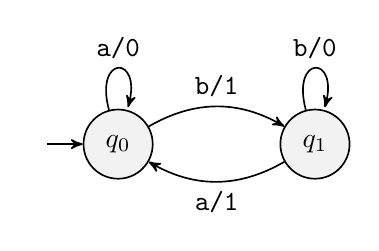
\begin{tikzpicture}
        \node[state,initial] (q0) {$q_0$};
        \node[state,right of=q0] (q1) {$q_1$};
        
        \draw (q0) edge[loop above] node {\tt a/0} (q0);
        \draw (q0) edge[bend left] node {\tt b/1} (q1);
        
        \draw (q1) edge[loop above] node {\tt b/0} (q1);
        \draw (q1) edge[bend left] node {\tt a/1} (q0);
    \end{tikzpicture}
\end{document}